\section{Трассировка лучей}
\begin{center}
    Конспект составил: \textit{Никита Луконенко}
\end{center}

\subsection{Введение в трассировку лучей}\label{1}

Представим, что у нас есть пейзаж, который мы хотим перерисовать. Какой самый простой способ это сделать?
Можно взять сетку от насекомых и две палки. Натянем между ними сетку и посмотрим через неё на пейзаж. Далее можно разлиновать холст на квадраты в соответствии с сеткой, и закрасить все квадратики теми цветами, которые мы увидим через сетку.
В результате мы получим примерно такой результат:

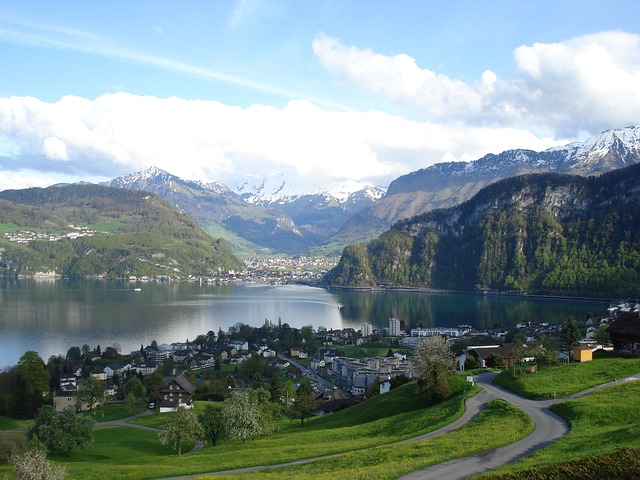
\includegraphics[width=5cm, height=4.8cm]{image1.png}
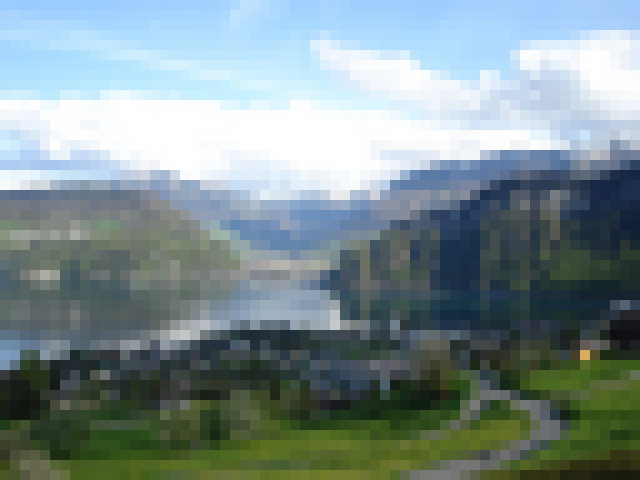
\includegraphics[width=5cm, height=4.8cm]{image2.png}

Запишем примитивный алгоритм трассировки лучей
\begin{lstlisting}
Place the eye and the frame as desired(1)
For each square on the canvas
    Determine which square on the grid corresponds(2) 
        to this square on the canvas
    Determine the color seen through that grid square(3)
    Paint the square with that color(4)
\end{lstlisting}

\subsection{Формализация процесса}\label{1}
Во-первых, мы будем считать, что точка обзора фиксирована. Точка обзора — это место, в котором располагается глаз в нашей аналогии, и оно обычно называется положением камеры; давайте назовём его $O = (O_x, O_y, O_z)$. Мы будем считать, что камера расположена в начале системы координат, то есть $O = (0, 0, 0)$.
Во-вторых, мы будем считать, что ориентация камеры тоже фиксирована, то есть камера всегда направлена в одно и то же место. Будем считать, что она смотрит вниз по положительной оси Z, положительная ось Y направлена вверх, а положительная ось X — вправо.
Также будем считать, что рамка имеет размеры $V_w$ и $V_h$, она фронтальна относительно положения камеры (то есть перпендикулярна $\vec{Z_+}$) и находится на расстоянии $d$, её стороны параллельны осям X и Y, и она центрирована относительно $\vec{Z_+}$.

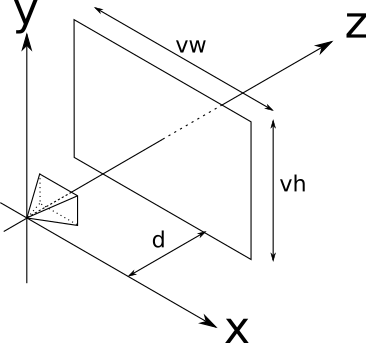
\includegraphics[width=5cm, height=4.8cm]{camera.png}

В сущности, мы будем рисовать на холсте всё то, что видим через окно просмотра. Важно, что размер окна просмотра и расстояние до камеры определяют угол видимости из камеры, называемый областью видимости (field of view) или для краткости FOV. У людей FOV по горизонтали составляет почти $180^\circ$, однако большая часть его составляет смутное периферическое зрение без ощущения глубины. В общем случае достоверные изображения получаются при использовании FOV $60^\circ$ в вертикальном и горизонтальном направлении; этого можно достичь, задав $V_w = V_h = d = 1$.

Вернемся к алгоритму, приведенному выше. Рассмотрим пункт 2, а затем сосредоточимся на более сложных способах реализации пункта 3.

\subsection{Из холста в окно просмотра}\label{1}
На шаге 2 нам нужно "Определить квадрат сетки, соответствующий этому пикселю". Мы знаем координаты пикселя на холсте (мы рисуем их все) — давайте назовём их $C_x$ и $C_y$. Оси окна просмотра соответствуют ориентации осей холста, а его центр соответствует центру окна просмотра, соответственно перейти от координат холста к координатам пространства можно простым изменением масштаба.

$V_x = C_x {V_w \over C_w}$,

$V_y = C_y {V_h \over C_h}$,

$V_z = d$.

На этом мы закончили шаг 2. Для каждого пикселя $(C_x, C_y)$ холста мы можем определить соответствующую точку окна просмотра $(V_x, V_y, V_z)$. На шаге 3 нам нужно определить, через какой цвет проходит свет $(V_x, V_y, V_z)$ с точки зрения обзора камеры $(O_x, O_y, O_z)$.

\subsection{Трассируем лучи}\label{1}
Какого цвета достигает свет $(O_x, O_y, O_z)$ после прохождения через $(V_x, V_y, V_z)$?

В реальном мире свет исходит из источника света (солнца, лампочки и т.д.), отражается от нескольких объектов и наконец достигает наших глаз. Мы можем попробовать симулировать путь каждого фотона, испущенного из симулированных источников света, но это будет невероятно затратно по времени (Эта техника называется трассировкой фотонов или распределением фотонов). Нам не только пришлось бы симулировать миллионы и миллионы фотонов, но и после прохождения через окно просмотра $(O_x, O_y, O_z)$ достигла бы только малая их часть.

Вместо этого мы будем трассировать лучи «в обратном порядке» — мы начнём с луча, находящегося на камере, проходящего через точку в окне просмотра и двигаясь, пока он не столкнётся с каким-нибудь объектом в сцене. Этот объект будет «виден» из камеры через эту точку окна просмотра. То есть в качестве первого приближения мы просто возьмём цвет этого объекта как «цвет света, прошедшего через эту точку»
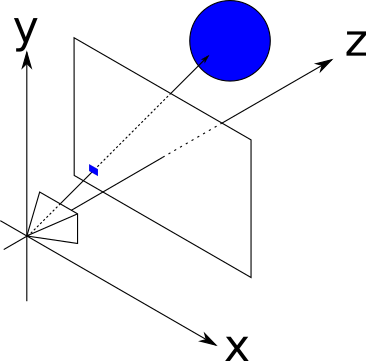
\includegraphics[width=5cm, height=4.8cm]{sphere_and_view.png}
\newpage
\subsubsection{Уравнение лучей}\label{2}

Мы знаем, что луч проходит через O, и мы знаем его направление

(из O в V), поэтому мы можем выразить любую точку P луча как

$P = O + t(V - O)$ где t — произвольное действительное число.

Обозначим $(V - O)$, то есть направление луча, как $\vec{D}$; тогда уравнение примет простой вид

$P = O + t\vec{D}$.
\subsubsection{Уравнение сферы}\label{3}
Теперь нам нужно добавить в сцену какие-нибудь объекты, чтобы лучи могли с чем-нибудь столкнуться. Мы можем выбрать в качестве строительного кирпичика сцен любой произвольный геометрический примитив; для трассировки лучей простейшим примитивом для математических манипуляций будет сфера.

Что такое сфера? Сфера — это множество точек, лежащих на постоянном расстоянии (называемом радиусом сферы) от фиксированной точки (называемой центром сферы):
Если C — центр сферы, а r — радиус сферы, то точки P на поверхности сферы удовлетворяют следующему уравнению:

$distance(P, C) = r$, $|P - C| = r$.

Длина вектора — это квадратный корень его скалярного произведения на себя:

$\sqrt{\langle P - C, P - C \rangle} = r$

И чтобы избавиться от квадратного корня,

$\langle P - C, P - C \rangle = r^2$

\subsubsection{Луч встречается со сферой}\label{4}
Теперь у нас есть два уравнения, одно из которых описывает точки сферы, а другое — точки луча:

$\langle P - C, P - C \rangle = r^2$

$P = O + t\vec{D}$

Точка P, в которой луч падает на сферу, является одновременно и точкой луча, и точкой на поверхности сферы, поэтому она должна удовлетворять обоим уравнениям одновременно. Заметьте, что единственная переменная в этих уравнениях — это параметр t, потому что O, $\vec{D}$, C и r заданы, а P — это точка, которую нам нужно найти.

Поскольку P — это одна и та же точка в обоих уравнениях, мы можем заменить P в первом на выражение для P во втором. Это даёт нам

$\langle O + t\vec{D} - C, O + t\vec{D} - C \rangle = r^2$.

Обозначим $\vec{OC} = O - C$.

$\langle \vec{OC} + t\vec{D}, \vec{OC} + t\vec{D} \rangle = r^2$

Затем мы разложим скалярное произведение на его компоненты, воспользовавшись его дистрибутивностью:

$\langle \vec{OC} + t\vec{D}, \vec{OC} \rangle + \langle \vec{OC} + t\vec{D}, t\vec{D} \rangle = r^2$

$\langle \vec{OC}, \vec{OC} \rangle + \langle t\vec{D}, \vec{OC} \rangle + \langle \vec{OC}, t\vec{D} \rangle + \langle t\vec{D}, t\vec{D} \rangle = r^2$

Преобразовав его немного, получим

$\langle t\vec{D}, t\vec{D} \rangle + 2\langle \vec{OC}, t\vec{D} \rangle + \langle \vec{OC}, \vec{OC} \rangle = r^2$

Переместив параметр t из скалярных произведений, а $r^2$ в другую часть уравнения, получим

$t^2 \langle \vec{D}, \vec{D} \rangle + t(2\langle \vec{OC}, \vec{D} \rangle) + \langle \vec{OC}, \vec{OC} \rangle - r^2 = 0$

Обозначим слагаемые полученного уравнения следующим образом:

$k_1 = \langle \vec{D}, \vec{D} \rangle$

$k_2 = 2\langle \vec{OC}, \vec{D} \rangle$

$k_3 = \langle \vec{OC}, \vec{OC} \rangle - r^2$

$k_1t^2 + k_2t + k_3 = 0$

$\{ t_1, t_2 \} = {{-k_2 \pm \sqrt{ {k_2}^2 -4k_1k_3} \over {2k_1}}}$

Полученное квадратное уравнение может не иметь решений, иметь одно двойное решение или два разных решения, в зависимости от значения дискриминанта ${k_2}^2 -4k_1k_3$. Это точно соответствует случаям, когда луч не пересекает сферу, луч касается сферы и луч входит и выходит из сферы:

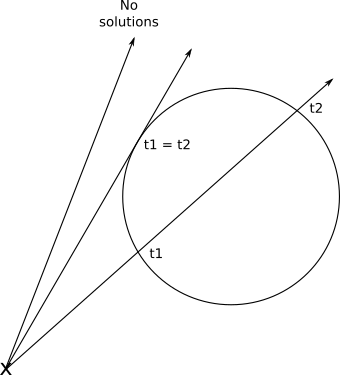
\includegraphics[width=5cm, height=4.8cm]{solutions.png}

Если мы возьмём значение t и вставим его в уравнение луча, то наконец получим точку пересечения P, соответствующее этому значению t.
Теперь мы можем попробовать отрендерить первую картинку.
\newpage
\subsection{Рендеринг первых сфер}
Псевдокод:
\begin{lstlisting}
O = <0, 0, 0>
for x in [-Cw/2, Cw/2] {
    for y in [-Ch/2, Ch/2] {
        D = CanvasToViewport(x, y)
        color = TraceRay(O, D, 1, inf)
        canvas.PutPixel(x, y, color)
    }
}

CanvasToViewport(x, y) {
    return (x*Vw/Cw, y*Vh/Ch, d)
}

TraceRay(O, D, t_min, t_max) {
    closest_t = inf
    closest_sphere = NULL
    for sphere in scene.Spheres {
        t1, t2 = IntersectRaySphere(O, D, sphere)
        if t1 in [t_min, t_max] and t1 < closest_t
            closest_t = t1
            closest_sphere = sphere
        if t2 in [t_min, t_max] and t2 < closest_t
            closest_t = t2
            closest_sphere = sphere
    }
    if closest_sphere == NULL
        return BACKGROUND_COLOR
    return closest_sphere.color
}

IntersectRaySphere(O, D, sphere) {
    C = sphere.center
    r = sphere.radius
    oc = O - C

    k1 = dot(D, D)
    k2 = 2*dot(OC, D)
    k3 = dot(OC, OC) - r*r

    discriminant = k2*k2 - 4*k1*k3
    if discriminant < 0:
        return inf, inf

    t1 = (-k2 + sqrt(discriminant)) / (2*k1)
    t2 = (-k2 - sqrt(discriminant)) / (2*k1)
    return t1, t2
}
\end{lstlisting}

\newpage
Зададим простую схему:

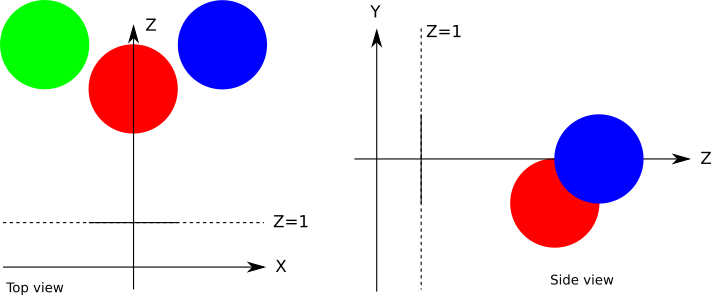
\includegraphics[width=12cm, height=4.8cm]{scene.png}

На псевдоязыке сцены она будет задана примерно так:

\begin{lstlisting}
viewport_size = 1 x 1
projection_plane_d = 1
sphere {
    center = (0, -1, 3)
    radius = 1
    color = (255, 0, 0)  
}
sphere {
    center = (2, 0, 4)
    radius = 1
    color = (0, 0, 255)  
}
sphere {
    center = (-2, 0, 4)
    radius = 1
    color = (0, 255, 0)  
}
\end{lstlisting}

Что получится:

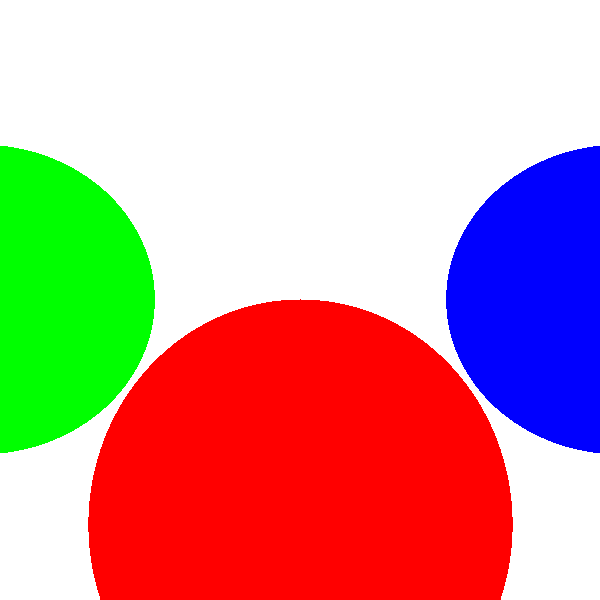
\includegraphics[width=7cm, height=4.8cm]{first_example.png}

\subsection{Освещение}
Введем несколько упрощений:
Всё освещение в контексте этого доклада имеет белый цвет. Это позволит нам охарактеризовать любой источник освещения единственным действительным числом i, называемым яркостью освещения.

Во-вторых, мы избавимся от атмосферы. Это значит, что освещение не становятся менее яркими, независимо от их дальности.
\subsubsection{Источники освещения}
\textbf{Точечные источники}

Точечный источник испускает свет из фиксированной точки в пространстве, называемой его позицией. Свет испускается равномерно во всех направлениях; именно поэтому его также называют всенаправленным освещением. Следовательно, точечный источник полностью характеризуется его позицией и яркостью.

Лампа накаливания — хороший пример из реального мира того, приближением чего является точечный источник освещения.

Зададим вектор $\vec{L}$ как направление из точки P в сцене к источнику освещения Q. Этот вектор, называемый световым вектором, просто равен $Q - P$. Заметьте, что поскольку Q фиксирована, а P может быть любой точкой сцены, то в общем случае $\vec{L}$ будет разным для каждой точки сцены.

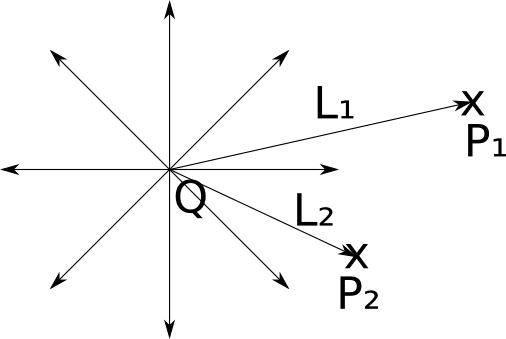
\includegraphics[width=7cm, height=4.8cm]{light_vectors.png}

\textbf{Направленные источники}

Нужен, когда расстояние до источника освещения слишком большое, и направление каждого луча света будет “почти” одинаковым.

Как и точечные источники, направленный источник имеет яркость, но в отличие от них, у него нет позиции. Вместо неё у него есть направление. Можно воспринимать его как бесконечно удалённый точечный источник, светящий в определённом направлении.

\textbf{Окружающее освещение}

Иногда лучи могут не попадать в места, которые в действительности надо осветить.
Можно считать каждый объект источником освещения, но это затратно по ресурсам.
Поэтому можно задать источник, который будет характеризоваться только яркостью.
Тогда общем случае будет только один источник окружающего освещения,
для вычисления освещенности точки вычислим кол-во света, которое вносит каждый источник, и сложим их.

Что произойдёт, когда луч света с направлением $\vec{L}$ из направленного или точечного источника падает на точку P какого-нибудь объекта в нашей сцене?

Интуитивно мы можем разбить объекты на два общих класса, в зависимости от того, как они ведут себя со светом: «матовые» и «блестящие». Поскольку большинство окружающих нас предметов можно считать «матовыми», то с них мы и начнём.

\subsubsection{Диффузное отражение}
Когда луч света падает на матовый объект, то из-за неровности его поверхности на микроскопическом уровне, он отражает луч в сцену равномерно во всех направлениях, то есть получается «рассеянное» («диффузное») отражение.

С другой стороны, количество отражённого света зависит от угла между лучом света и поверхностью. Интуитивно это понятно — энергия, переносимая лучом, в зависимости от угла должна распределиться по меньшей или большей поверхности, то есть энергия на единицу площади, отражённая в сцену, будет соответственно выше или ниже:

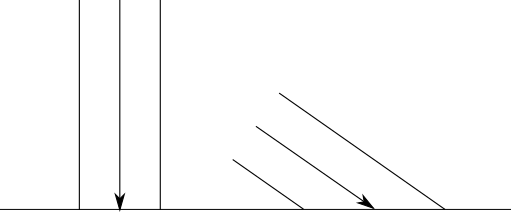
\includegraphics[width=7cm, height=4.8cm]{light_vectors1.png}

Итак, луч света с направлением $\vec{L}$ и яркостью $I$ падает на поверхность с нормалью $\vec{N}$.

Для геометрической аналогии давайте представим яркость света как «ширину» луча. Его энергия распределяется по поверхности размером $A$. Когда $\vec{N}$ и $\vec{L}$ имеют одно направление, то есть луч перпендикулярен поверхности, $I = A$, а это значит, что энергия, отражённая на единицу площади равна падающей энергии на единицу площади; <${I \over A} = 1$. С другой стороны, когда угол между $\vec{L}$ и $\vec{N}$ приближается к $90^\circ$, $A$ приближается к $\infty$, то есть энергия на единицу площади приближается к 0; $\lim_{A \to \infty} {I \over A} = 0$.

Ситуация отображена на схеме ниже. Мы знаем $\vec{N}$, $\vec{L}$ и $P$; я добавил углы $\alpha$ и $\beta$, а также точки $Q$, $\vec{R}$ и $S$, чтобы сделать связанные с этой схемой записи проще.

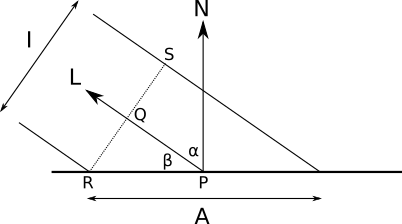
\includegraphics[width=8.5cm, height=4.8cm]{light_vectors2.png}

Поскольку технически луч света не имеет ширины, поэтому мы будем считать, что всё происходит на бесконечно малом плоском участке поверхности. Даже если это поверхность сферы, то рассматриваемая область настолько бесконечно мала, что она почти плоская относительно размера сферы, так же как Земля выглядит плоской при малых масштабах.

Луч света с шириной $I$ падает на поверхность в точке $P$ под углом $\beta$. Нормаль в точке $P$ равна $\vec{N}$, а энергия, переносимая лучом, распределяется по $A$. Нам нужно вычислить ${I \over A}$.

Будем считать $SR$ «шириной» луча. По определению, она перпендикулярна $\vec{L}$, который также является направлением $PQ$. Поэтому $PQ$ и $QR$ образуют прямой угол, превращая $PQR$ в прямоугольный треугольник.

Один из углов $PQR$ равен $90^\circ$, а другой — $\beta$. Тогда третий угол равен $90^\circ - \beta$. Но нужно заметить, что $\vec{N}$ и $PR$ тоже образуют прямой угол, то есть $\alpha + \beta$ тоже должны быть $90^\circ$. Следовательно, $\widehat{QRP} = \alpha$
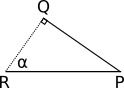
\includegraphics[width=6cm, height=4.8cm]{triangle.png}

Давайте рассмотрим треугольник $PQR$. Его углы равны $\alpha$, $\beta$ и $90^\circ$. Сторона $QR$ равна $I \over 2$, а сторона $PR$ равна $A \over 2$.

По определению $cos(\alpha) = {QR \over PR}$; заменяем $QR$ на $I \over 2$, а $PR$ на $A \over 2$, и получаем:

$cos(\alpha) = { {I \over 2} \over {A \over 2} }$  что преобразуется в

$cos(\alpha) = {I \over A}$

$\alpha$ — это угол между $\vec{N}$ и $\vec{L}$, то есть $cos(\alpha)$ можно выразить как

$cos(\alpha) = {{\langle \vec{N}, \vec{L} \rangle} \over {|\vec{N}||\vec{L}|}}$

${I \over A} = {{\langle \vec{N}, \vec{L} \rangle} \over {|\vec{N}||\vec{L}|}}$

Итак, мы получили очень простое уравнение, связывающее отражённую часть света с углом между нормалью к поверхности и направлением света.

Заметьте, что при углах больше $90^\circ$ значение $cos(\alpha)$ становится отрицательным. Если мы не задумываясь используем это значение, то в результате получим источники света, вычитающие свет. Это не имеет никакого физического смысла; угол больше $90^\circ$ просто означает, что свет на самом деле достигает задней части поверхности, и не вносит свой вклад в освещение освещаемой точки. То есть если $cos(\alpha)$ становится отрицательным, то мы считаем его равным $0$.

Уравнение диффузного отражения

Теперь мы можем сформулировать уравнение для вычисления полного количества света, полученного точкой $P$ с нормалью $\vec{N}$ в сцене с окружающим освещением яркостью $I_A$ и $n$ точечных или направленных источников света с яркостью $I_n$ и световыми векторами $\vec{L_n}$ или известными (для направленных источников), или вычисленными для P (для точечных источников):

$I_P = I_A + \sum_{i = 1}^{n} I_i {{\langle \vec{N}, \vec{L_i} \rangle} \over {|\vec{N}||\vec{L_i}|}}$

Стоит снова повторить, что члены, в которых $\langle \vec{N}, \vec{L_i} \rangle < 0$ не должны прибавляться к освещённости точки.

\subsubsection{Нормали сферы}

Вектор нормали любой точки сферы лежит на прямой, проходящей через центр сферы. То есть если центр сферы — это $C$, то направление нормали в точки $P$ равно $P - C$:

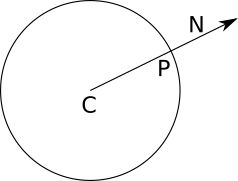
\includegraphics[width=6.5cm, height=4.8cm]{sphere.png}

Кроме перпендикулярности к поверхности, нормаль должна быть единичным вектором; это было бы справедливо, если бы радиус сферы был равен $1$, что не всегда верно. Для вычисления самой нормали нам нужно разделить вектор на его длину, получив таким образом длину $1$:

$\vec{N} = {{P - C} \over {|P - C|}}$

\subsubsection{Рендеринг с диффузным отражением}
\begin{lstlisting}
light {
    type = ambient
    intensity = 0.2
}
light {
    type = point
    intensity = 0.6
    position = (2, 1, 0)
}
light {
    type = directional
    intensity = 0.2
    direction = (1, 4, 4)
}
\end{lstlisting}

Заметьте, что яркость удобно суммируется в $1.0$, потому что из уравнения освещения следует, что никакая точка не может иметь яркость света выше, чем единица. Это значит, что у нас не получатся области со «слишком большой выдержкой».

Уравнение освещения довольно просто преобразовать в псевдокод:
\begin{lstlisting}
ComputeLighting(P, N) {
    i = 0.0
    for light in scene.Lights {
        if light.type == ambient {
            i += light.intensity
        } else {
            if light.type == point
                L = light.position - P
            else
                L = light.direction

            n_dot_l = dot(N, L)
            if n_dot_l > 0
                i += light.intensity*n_dot_l/(length(N)*length(L))
        }
    }
    return i
}
\end{lstlisting}

И единственное, что осталось — использовать ComputeLighting в TraceRay. Мы заменим строку, возвращающую цвет сферы

\begin{lstlisting}
    return closest_sphere.color
\end{lstlisting}

на этот фрагмент:

\begin{lstlisting}
    P = O + closest_t*D  
    N = P - closest_sphere.center 
    N = N / length(N)
    return closest_sphere.color*ComputeLighting(P, N)
\end{lstlisting}

\newpage
Если запустить рендерер, то получится такое изображение:

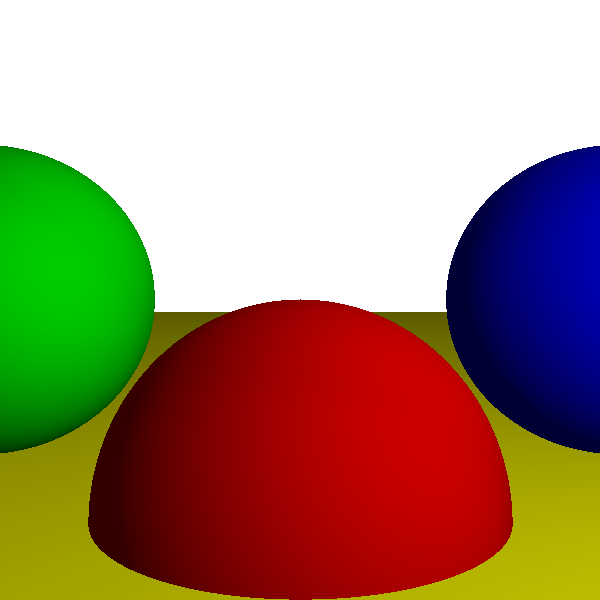
\includegraphics[width=13cm, height=11.8cm]{second_example.png}

Теперь сферы приобрели объем.

\subsubsection{Отражение от гладкой поверхности}

Теперь мы обратим своё внимание на «блестящие» объекты. В отличие от «матовых» объектов, «блестящие» меняют свой внешний вид, когда смотришь на них под разными углами.

Возьмём бильярдный шар или только что вымытый автомобиль. В таких объектах проявляется особый шаблон распространения света, обычно с яркими областями, которые как будто движутся, когда вы ходите вокруг них. В отличие от матовых объектов, то, как вы воспринимаете поверхность этих объектов, на самом деле зависит от точки обзора.

Заметьте, что красные бильярдные шары остаются красными, если вы отойдёте на пару шагов назад, но яркое белое пятно, дающее им «блестящий» вид, похоже, двигается. Это значит, что новый эффект не заменяет диффузное отражение, а дополняет его.

Как мы видели в предыдущем разделе, когда луч света падает на поверхность матового объекта, он равномерно рассеивается назад в сцену во всех направлениях. Интуитивно понятно, что так происходит из-за неровности поверхности объекта, то есть на микроскопическом уровне она похожа на множество мелких поверхностей, направленных в случайных направлениях:

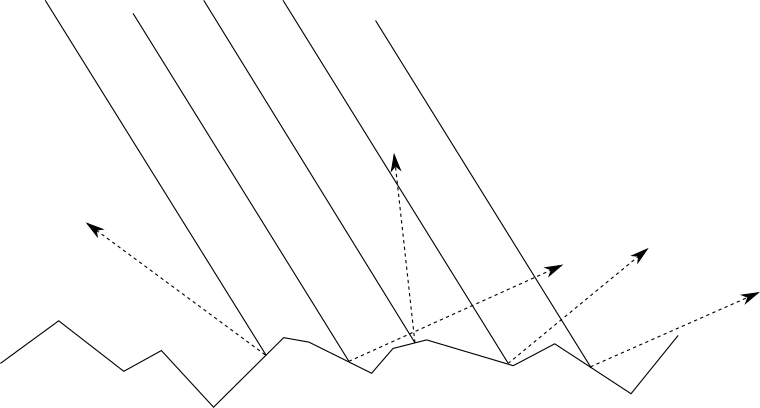
\includegraphics[width=5cm, height=4.8cm]{light_vectors3.png}

Когда луч света падает на зеркало, он отражается в единственном направлении, которое симметрично углу падения относительно нормали зеркала. Если мы назовём направление отражённого света $\vec{R}$ и условимся, что $\vec{L}$ указывает на источник света, то получим такую ситуацию:

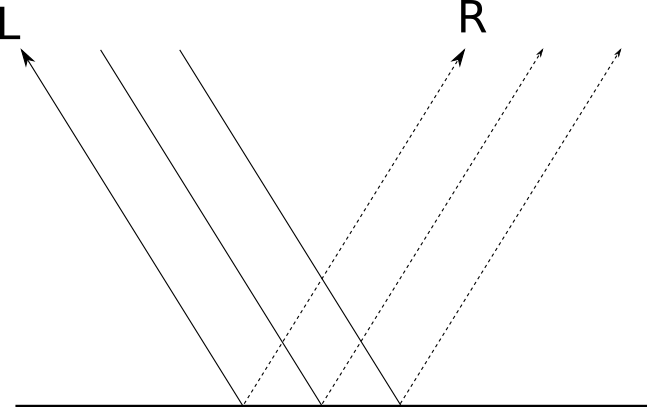
\includegraphics[width=5cm, height=4.8cm]{light_vectors4.png}

В зависимости от степени «отполированности» поверхности, она более или менее похожа на зеркало.

Для идеально отполированного зеркала падающий луч света $\vec{L}$ отражается в единственном направлении $\vec{R}$. Именно это позволяет нам чётко видеть объекты в зеркале: для каждого падающего луча $\vec{L}$ есть единственный отражённый луч $\vec{R}$. Но не каждый объект отполирован идеально; хотя большая часть света отражается в направлении $\vec{R}$, часть его отражается в направлениях, близких к $\vec{R}$; чем ближе к $\vec{R}$, тем больше света отражается в этом направлении.

«Блеск» объекта определяет то, насколько быстро отражённый свет уменьшается при отдалении от $\vec{R}$:

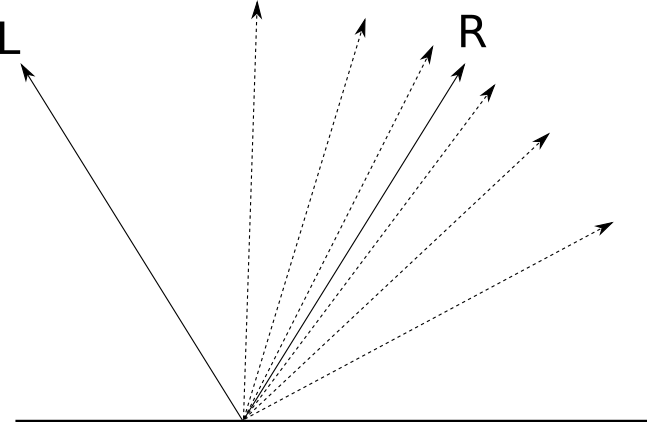
\includegraphics[width=7cm, height=4.8cm]{light_vectors5.png}

Нас интересует то, как выяснить, какое количество света от $\vec{L}$ отражается обратно в направлении нашей точки обзора (потому что это свет, который мы используем для определения цвета каждой точки). Если $\vec{V}$ — это «вектор обзора», указывающий из $P$ в камеру, а $\alpha$ — угол между $\vec{R}$ и $\vec{V}$, то вот, что мы имеем:

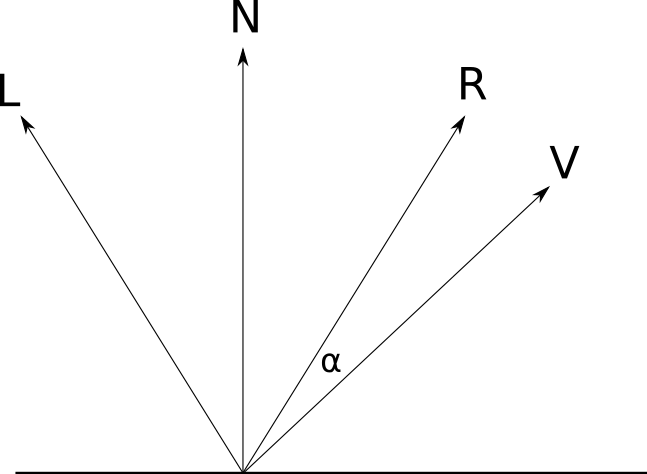
\includegraphics[width=7cm, height=4.8cm]{light_vectors6.png}

При $\alpha = 0^\circ$ отражается весь свет. При $\alpha = 90^\circ$ свет не отражается. Как и в случае с диффузным отражением, нам нужно математическое выражение для определения того, что происходит при промежуточных значениях $\alpha$.

\newpage
\subsubsection{Моделирование «зеркального» отражения}

Давайте возьмём $cos(\alpha)$. У него есть хорошие свойства: $cos(0) = 1$, $cos(\pm 90) = 0$, а значения постепенно уменьшаются от $0$ до $90$:

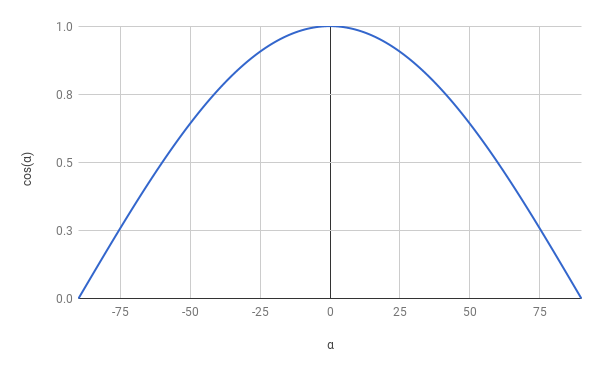
\includegraphics[width=10cm, height=8cm]{cos.png}

Блеск — мера того, насколько быстро функция отражения уменьшается при увеличении $\alpha$. Очень простой способ получения различных кривых блеска заключается в вычислении степени $cos(\alpha$ некоего положительного показателя $s$. Поскольку $0 \le cos(\alpha) \le 1$, то очевидно, что $0 \le cos(\alpha)^s \le 1$; то есть $cos(\alpha)^s$ ведёт себя точкно так же, как $cos(\alpha$, только «уже»(см. на график). Вот $cos(\alpha)^s$ для разных значений $s$:

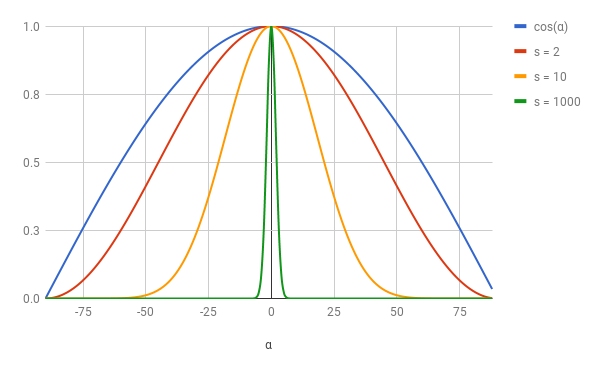
\includegraphics[width=10cm, height=6cm]{cos1.png}

Чем больше значение $s$, тем «уже» становится функция в окрестностях $0$, и тем более блестящим выглядит объект.

$s$ обычно называют показателем отражения, и он является свойством поверхности. Поскольку модель не основана на физической реальности, значения $s$ можно определить только методом проб и ошибок, то есть настраивая значения до тех пор, пока они не начнут выглядеть «естественно» (Примечание: для использования модели на основе физики см. двулучевую функцию отражательной способности (ДФОС)).

Объединим всё вместе. Луч $\vec{L}$ падает на поверхность в точке $P$, где нормаль равна $\vec{N}$, а показатель отражения — $s$.

Количество света, которое отразится в направлении обзора $\vec{V}$ равно $cos(\alpha)^s$, где $\alpha$ — это угол между $\vec{V}$ и $\vec{R}$, который в свою очередь является $\vec{L}$, отражённым относительно $\vec{N}$. То есть первым шагом будет вычисление $\vec{R}$ из $\vec{N}$ и $\vec{L}$.

Мы можем разложить $\vec{L}$ на два вектора $\vec{L_P}$ и $\vec{L_N}$, таких, что $\vec{L} = \vec{L_P} + \vec{L_N}$, где $\vec{L_N}$ параллелен $\vec{N}$, а $\vec{L_P}$ перпендикулярен $\vec{N}$:

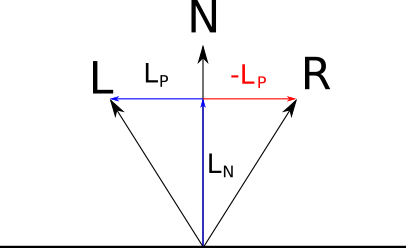
\includegraphics[width=10cm, height=6cm]{proections.png}

$\vec{L_N}$ — это проекция $\vec{L}$ на $\vec{N}$; по свойствам скалярного произведения и исходя из того, что $|\vec{N}| = 1$, длина этой проекции равна $\langle \vec{N}, \vec{L} \rangle$. Мы определили, что $\vec{L_N}$ будет параллелен $\vec{N}$, поэтому $\vec{L_N} = \vec{N} \langle \vec{N}, \vec{L} \rangle$.

Поскольку $\vec{L} = \vec{L_P} + \vec{L_N}$, мы можем сразу получить $\vec{L_P} = \vec{L} - \vec{L_N} = \vec{L} - \vec{N} \langle \vec{N}, \vec{L} \rangle$.

Теперь посмотрим на $\vec{R}$; поскольку он симметричен $\vec{L}$ относительно $\vec{N}$, его компонент, параллельный $\vec{N}$, тот же, что и у $\vec{L}$, а перпендикулярный компонент противоположен компоненту $\vec{L}$; то есть $\vec{R} = \vec{L_N} - \vec{L_P}$:

Подставляя полученные ранее выражения, мы получим

$\vec{R} = \vec{N} \langle \vec{N}, \vec{L} \rangle - \vec{L} + \vec{N} \langle \vec{N}, \vec{L} \rangle$

и немного упростив, получаем

$\vec{R} = 2\vec{N} \langle \vec{N}, \vec{L} \rangle - \vec{L}$

Теперь мы готовы записать уравнение «зеркального» отражения:

$\vec{R} = 2\vec{N} \langle \vec{N}, \vec{L} \rangle - \vec{L}$

$I_S = I_L \left( {{\langle \vec{R}, \vec{V} \rangle} \over {|\vec{R}||\vec{V}|}} \right)^s$

Как и в случае диффузного освещения, $cos(\alpha)$ может быть отрицательным, и мы снова должны это игнорировать. Кроме того, не каждый объект должен быть блестящим; для таких объектов (который мы будем представлять через $s = -1$) значение «зеркальности» вообще не будет вычисляться.

\subsubsection{Моделирование «зеркального» отражения}

Добавим в сцену «зеркальные» отражения. Внесём некоторые изменения в саму сцену:

\begin{lstlisting}
sphere {
    center = (0, -1, 3)
    radius = 1
    color = (255, 0, 0)  
    specular = 500  
}
sphere {
    center = (-2, 1, 3)
    radius = 1
    color = (0, 0, 255)  
    specular = 500  
}
sphere {
    center = (2, 1, 3)
    radius = 1
    color = (0, 255, 0)  
    specular = 10  
}
sphere {
    color = (255, 255, 0)  
    center = (0, -5001, 0)
    radius = 5000
    specular = 1000  
}
\end{lstlisting}

В коде нам нужно изменить ComputeLighting, чтобы он при необходимости вычислял значение «зеркальности» и прибавлял его к общему освещению. Заметьте, что теперь ему требуются $\vec{V}$ и $s$:

\begin{lstlisting}
ComputeLighting(P, N, V, s) {
    i = 0.0
    for light in scene.Lights {
        if light.type == ambient {
            i += light.intensity
        } else {
            if light.type == point
                L = light.position - P
            else
                L = light.direction


            n_dot_l = dot(N, L)
            if n_dot_l > 0
                i += light.intensity*n_dot_l/(length(N)*length(L))


            if s != -1 {
                R = 2*N*dot(N, L) - L
                r_dot_v = dot(R, V)
                if r_dot_v > 0
                    i += light.intensity
                        *pow(r_dot_v/(length(R)*length(V)), s)
            }
        }
    }
    return i
}
\end{lstlisting}

Также нужно изменить TraceRay, чтобы он передавал новые параметры ComputeLighting. $s$ очевиден; он берётся из данных сферы. У нас уже есть вектор, направленный из камеры к объекту — это $\vec{D}$, направление трассируемого луча. То есть $\vec{V}$ — это просто $-\vec{D}$.

\begin{lstlisting}
TraceRay(O, D, t_min, t_max) {
    closest_t = inf
    closest_sphere = NULL
    for sphere in scene.Spheres {
        t1, t2 = IntersectRaySphere(O, D, sphere)
        if t1 in [t_min, t_max] and t1 < closest_t
            closest_t = t1
            closest_sphere = sphere
        if t2 in [t_min, t_max] and t2 < closest_t
            closest_t = t2
            closest_sphere = sphere
    }
    if closest_sphere == NULL
        return BACKGROUND_COLOR

    P = O + closest_t*D  
    N = P - closest_sphere.center  
    N = N / length(N)
    return closest_sphere.color*ComputeLighting(P, N, 
            -D, sphere.specular)
}
\end{lstlisting}

Если мы запустим рендерер, то у нас получится следующая картинка:

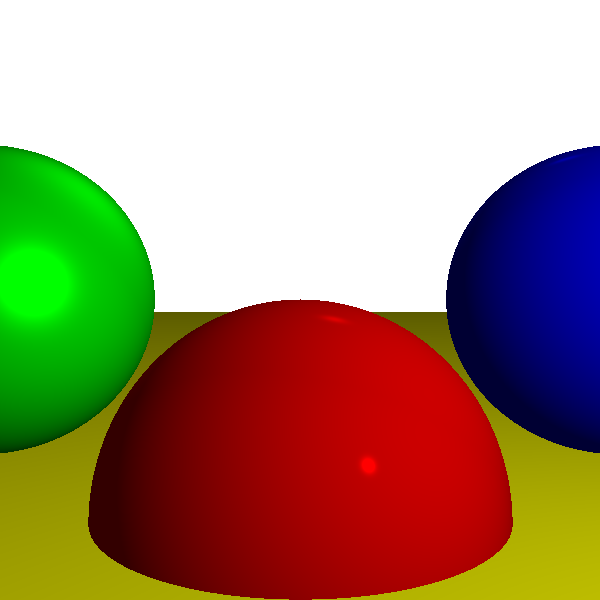
\includegraphics[width=13cm, height=11.8cm]{third_example.png}

\newpage
\subsection{Тени}

Там, где есть свет и объекты, должны быть и тени.

В предыдущем разделе нас интересовали углы и вектора, но мы рассматривали только источник света и точку, которую нам нужно раскрасить, и полностью игнорировали всё остальное, что происходит в сцене — например, попавшийся на пути объект.

Мы хотим выделить два следующих случая:

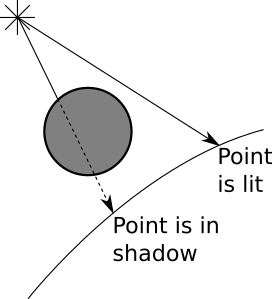
\includegraphics[width=4.8cm, height=5cm]{shadows1.png}

$P$; это точка, которая нас интересует. $\vec{L}$; это часть определения источника освещения. Имея $P$ и $\vec{L}$, мы можем задать луч, а именно $P + t\vec{L}$, который проходит из точки до бесконечно отдалённого источника освещения. Пересекает ли этот луч другой объект? Если нет, то между точкой и источником ничего нет, то есть мы можем вычислить освещённость от этого источника и прибавить его к общей освещённости. Если пересекает, то мы игнорируем этот источник.

Мы уже знаем, как вычислить ближайшее пересечение между лучом и сферой; мы используем его для трассировки лучей от камеры. Но вместо того, чтобы начинаться с камеры, лучи испускаются из $P$. Направление равно не $(V - O)$, а $\vec{L}$. И нас интересуют пересечения со всем после $P$ на бесконечное расстояние; это значит, что $t_{min} = 0$ и $t_{max} = +\infty$.

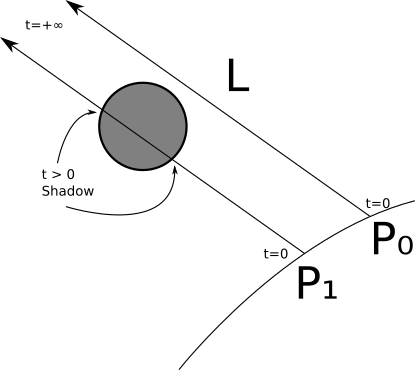
\includegraphics[width=4.8cm, height=5cm]{shadows2.png}
\newpage
Мы можем обрабатывать точечные источники очень похожим образом, но с двумя исключениями. Во-первых, не задан $\vec{L}$, но его очень просто вычислить из позиции источника и $P$. Во-вторых, нас интересуют любые пересечения, начиная с $P$, но только до $L$ (в противном случае, объекты за источником освещения могли бы создавать тени); то есть в этом случае $t_{min} = 0$ и $t_{max} = 1$.

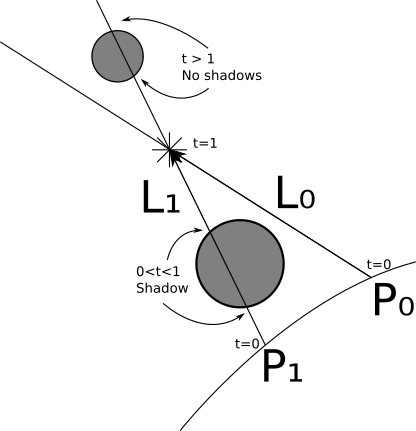
\includegraphics[width=6.8cm, height=7cm]{shadows3.png}

Пограничный случай, который нужно рассмотреть.
Мы хотим найти пересечение луча с каким либо объектом, но хотим избежать ситуации, когда точка объекта бросает тень на саму себя.
Геометрически, мы хотим сделать так, чтобы луч начинается немного вдали от поверхности, то есть рядом с $P$, но не точно в $P$. То есть для направленных источников интервал будет $[\epsilon, +\infty]$, а для точечных — $[\epsilon, 1]$.

\textbf{Рендеринг с тенями}

\begin{lstlisting}
ClosestIntersubsection(O, D, t_min, t_max) {
    closest_t = inf
    closest_sphere = NULL
    for sphere in scene.Spheres {
        t1, t2 = IntersectRaySphere(O, D, sphere)
        if t1 in [t_min, t_max] and t1 < closest_t
            closest_t = t1
            closest_sphere = sphere
        if t2 in [t_min, t_max] and t2 < closest_t
            closest_t = t2
            closest_sphere = sphere
    }
    return closest_sphere, closest_t
}
\end{lstlisting}

В результате TraceRay получается гораздо проще:

\begin{lstlisting}
TraceRay(O, D, t_min, t_max) {
    closest_sphere, closest_t = ClosestIntersubsection(O, 
                                D, t_min, t_max)

    if closest_sphere == NULL
        return BACKGROUND_COLOR

    P = O + closest_t*D  # Compute intersubsection
    N = P - closest_sphere.center  
    N = N / length(N)
    return closest_sphere.color*ComputeLighting(P, N, 
            -D, sphere.specular)
}
\end{lstlisting}

Теперь нам нужно добавить в ComputeLighting проверку тени:

\begin{lstlisting}
ComputeLighting(P, N, V, s) {
    i = 0.0
    for light in scene.Lights {
        if light.type == ambient {
            i += light.intensity
        } else {
            if light.type == point {
                L = light.position - P
                t_max = 1
            } else {
                L = light.direction
                t_max = inf
            }

            
            shadow_sphere, shadow_t = ClosestIntersubsection(P, L, 
                                        0.001, t_max)
            if shadow_sphere != NULL
                continue

            
            n_dot_l = dot(N, L)
            if n_dot_l > 0
                i += light.intensity*n_dot_l/(length(N)*length(L))

            
            if s != -1 {
                R = 2*N*dot(N, L) - L
                r_dot_v = dot(R, V)
                if r_dot_v > 0
                    i += light.intensity*pow(r_dot_v/(length(R)
                        *length(V)), s)
            }
        }
    }
    return i
}
\end{lstlisting}

Так будет выглядеть наша заново отрендеренная сцена:

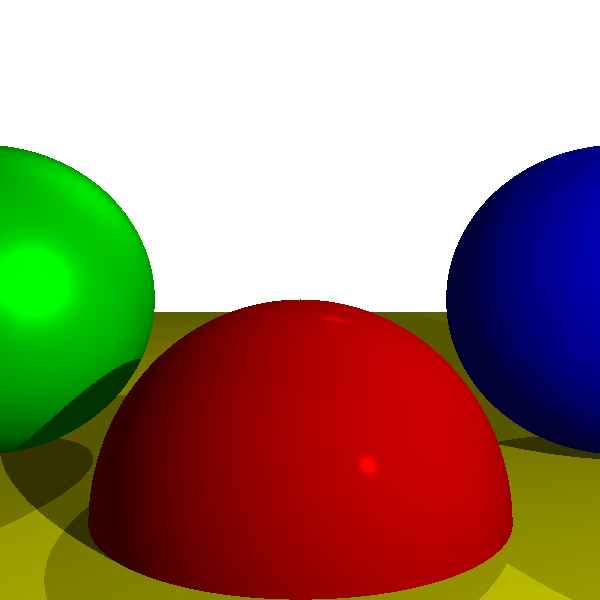
\includegraphics[width=13cm, height=11.8cm]{shadows4.png}

\subsection{Отражение}
Когда мы смотрим в зеркало, то видим лучи света, отражающиеся от зеркала. Лучи света отражаются симметрично относительно нормали поверхности:

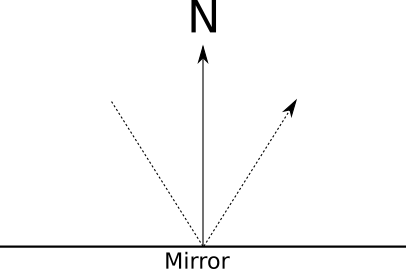
\includegraphics[width=8cm, height=5cm]{reflection.png}

Нам нужно — вычислить направление отражённого луча и выяснить, каким был цвет света, падающего из этого направления.
У нас уже есть функция TraceRay, но она возвращает цвет объекта, с которым сталкивается вектор из камеры.
Нужно модифицировать её, чтобы она работала для лучей из других объектов.
Начинаем с основного цикла TraceRay, чтобы увидеть, что «видит» луч, испущенный из камеры. Если TraceRay определяет, что луч видит отражающий объект, то он просто должен вычислить направление отражённого луча и вызвать сам себя.

Нам необходимо учесть ситуацию, при которой возникает бесконечная рекурсия.
Есть очевидное условие выхода: когда луч или падает на неотражающий объект, или когда он ни на что не падает. Но есть ситуация, когда два отражающих объекта появляются друг напротив друга. Чтобы не уйти в бесконечную рекурсию в этом случае добавим максимальную глубину рекурсии.
Давайте назовём её $r$. При $r = 0$, то видим объекты, но без отражений. При $r = 1$ Мы видим некоторые объекты и отражения некоторых объектов. При $r = 2$ мы видим некоторые объекты, отражения некоторых объектов и отражения некоторых отражений некоторых объектов. И так далее. В общем случае, нет особого смысла уходить вглубь больше чем на 2-3 уровня, потому что на этом этапе разница уже едва заметна.
Мы создадим ещё одно разграничение. «Отражаемость» не должна иметь значение «есть или нет» — объекты могут быть частично отражающими и частично цветными. Мы назначим каждой поверхности число от $0$ до $1$, определяющее её отражаемость. После чего мы будем смешивать локально освещённый цвет и отражённый цвет пропорционально этому числу.

Луч начинается с поверхности объекта, точки $P$. Направление луча — это направление света, отразившегося от $P$; в TraceRay у нас есть $\vec{D}$, то есть направление от камеры к $P$, противоположное движению света, то есть направление отражённого луча будет $\vec{-D}$, отражённый относительно $\vec{N}$. Аналогично тому, что происходит с тенями, мы не хотим, чтобы объекты отражали сами себя, поэтому $t_{min} = \epsilon$. Мы хотим видеть объекты отражёнными вне зависимости от того, насколько они отдалены, поэтому $t_{max} = +\infty$. И последнее — предел рекурсии на единицу меньше, чем предел рекурсии, в котором мы находимся в текущий момент.

\textbf{Рендеринг с отражением}

Давайте добавим к коду трассировщика лучей отражение.

Как и ранее, в первую очередь мы изменяем сцену:
\begin{lstlisting}
sphere {
    center = (0, -1, 3)
    radius = 1
    color = (255, 0, 0) 
    specular = 500  
    reflective = 0.2  
}
sphere {
    center = (-2, 1, 3)
    radius = 1
    color = (0, 0, 255) 
    specular = 500  
    reflective = 0.3  
}
sphere {
    center = (2, 1, 3)
    radius = 1
    color = (0, 255, 0)  
    specular = 10  
    reflective = 0.4  
}
sphere {
    color = (255, 255, 0)  
    center = (0, -5001, 0)
    radius = 5000
    specular = 1000  
    reflective = 0.5  
}
\end{lstlisting}

Мы используем формулу «луча отражения» в паре мест, поэтому может избавиться от неё. Она получает луч $\vec{R}$ и нормаль $\vec{N}$, возвращая $\vec{R}$, отражённый относительно $\vec{N}$:

\begin{lstlisting}
ReflectRay(R, N) {
    return 2*N*dot(N, R) - R;
}
\end{lstlisting}

Единственным изменением в ComputeLighting является замена уравнения отражения на вызов этого нового ReflectRay.
В основной метод внесено небольшое изменение — нам нужно передать TraceRay верхнего уровня предел рекурсии:

\begin{lstlisting}
color = TraceRay(O, D, 1, inf, recursion_depth)
\end{lstlisting}

Константе recursion\_depth можно задать разумное значение, например, 3 или 5.

Единственные важные изменения происходят ближе к концу TraceRay, где мы рекурсивно вычисляем отражения:

\begin{lstlisting}
TraceRay(O, D, t_min, t_max, depth) {
    closest_sphere, closest_t = ClosestIntersubsection(O, 
                                D, t_min, t_max)

    if closest_sphere == NULL
        return BACKGROUND_COLOR

    
    P = O + closest_t*D  
    N = P - closest_sphere.center  
    N = N / length(N)
    local_color = closest_sphere.color*ComputeLighting(P, N, 
                    -D, sphere.specular)

    
    r = closest_sphere.reflective
    if depth <= 0 or r <= 0:
        return local_color

    
    R = ReflectRay(-D, N)
    reflected_color = TraceRay(P, R, 0.001, inf, depth - 1)

    return local_color*(1 - r) + reflected_color*r
}
\end{lstlisting}

Итоговый результат выглядит следующим образом:

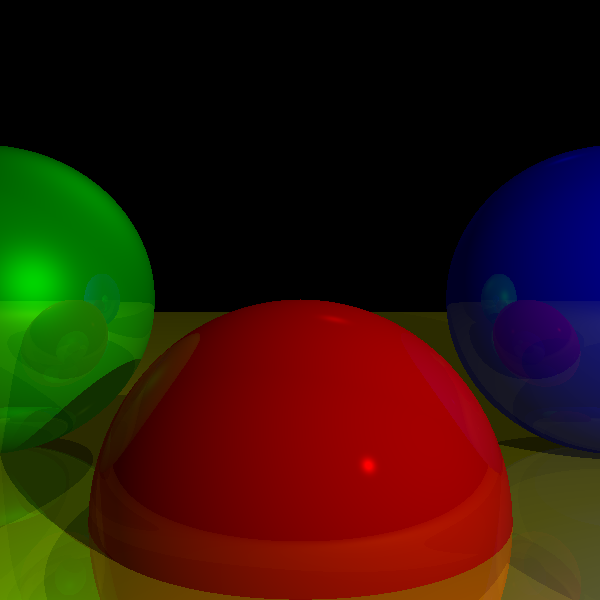
\includegraphics[width=13.8cm, height=11cm]{fourth_example.png}
